\documentclass[11pt,a4paper]{article}

\usepackage{datetime}
\usepackage{graphicx}
\usepackage{subcaption}

\usepackage{hyperref}

\hypersetup{
    colorlinks=true,
    linkcolor=blue,
    filecolor=magenta,      
    urlcolor=cyan,
}


\title{Chapter 3 Lab Work: Processes and Threads}
\newdate{date}{21}{04}{2020}
\date{\displaydate{date}}
\author{Nguyen Ngoc Lam - 20162316}

\begin{document}
	\pagenumbering{gobble}
  	\maketitle
  	\newpage
  	\tableofcontents
  	\newpage
  	
  	\section{New File on ChatRoomApp folder}
  	The new file in said folder is package.json. This file holds various metadata relevant to the project. This file is used to give information to npm that allows it to identify the project as well as handle the project's dependencies. It can also contain other metadata such as a project description, the version of the project in a particular distribution, license information, even configuration data - all of which can be vital to both npm and to the end users of the package. The package.json file is normally located at the root directory of a Node.js project.
  	\begin{figure}[h!]
		\centering
  		\begin{subfigure}[b]{0.4\linewidth}
  		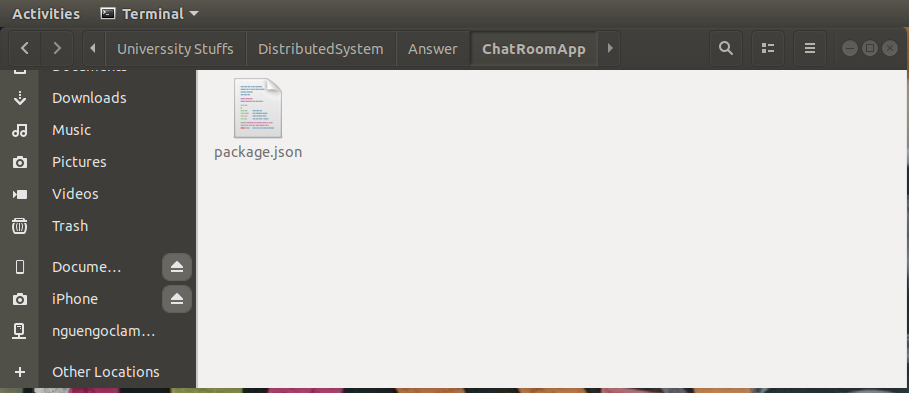
\includegraphics[width=\linewidth]{files-expl-chat.png}
    		\caption{File Explorer}
  		\end{subfigure}
  		\begin{subfigure}[b]{0.4\linewidth}
    		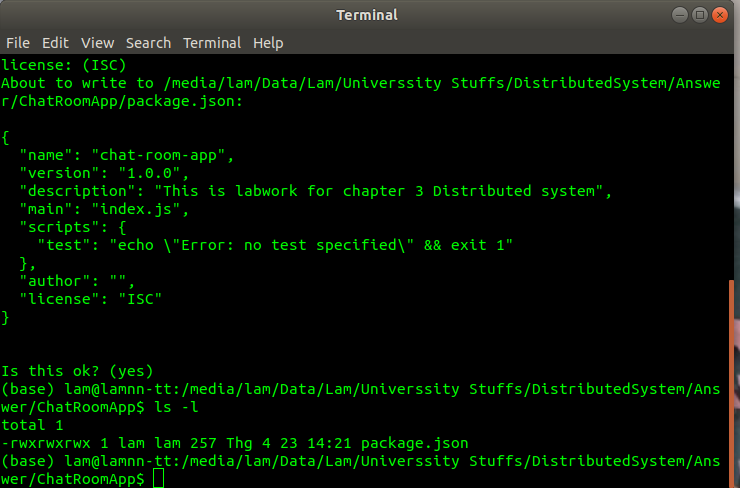
\includegraphics[width=\linewidth]{term-chat.png}
    		\caption{In terminal}
  		\end{subfigure}
  		\caption{New file}
  		\label{fig:pack}
	\end{figure}
	
	\section{Message On Port 3000}
	If you access to '127.0.0.1:3000' (or localhost:3000), the display message on the screen is hello world in plain text.
	\begin{figure}[h!]
  		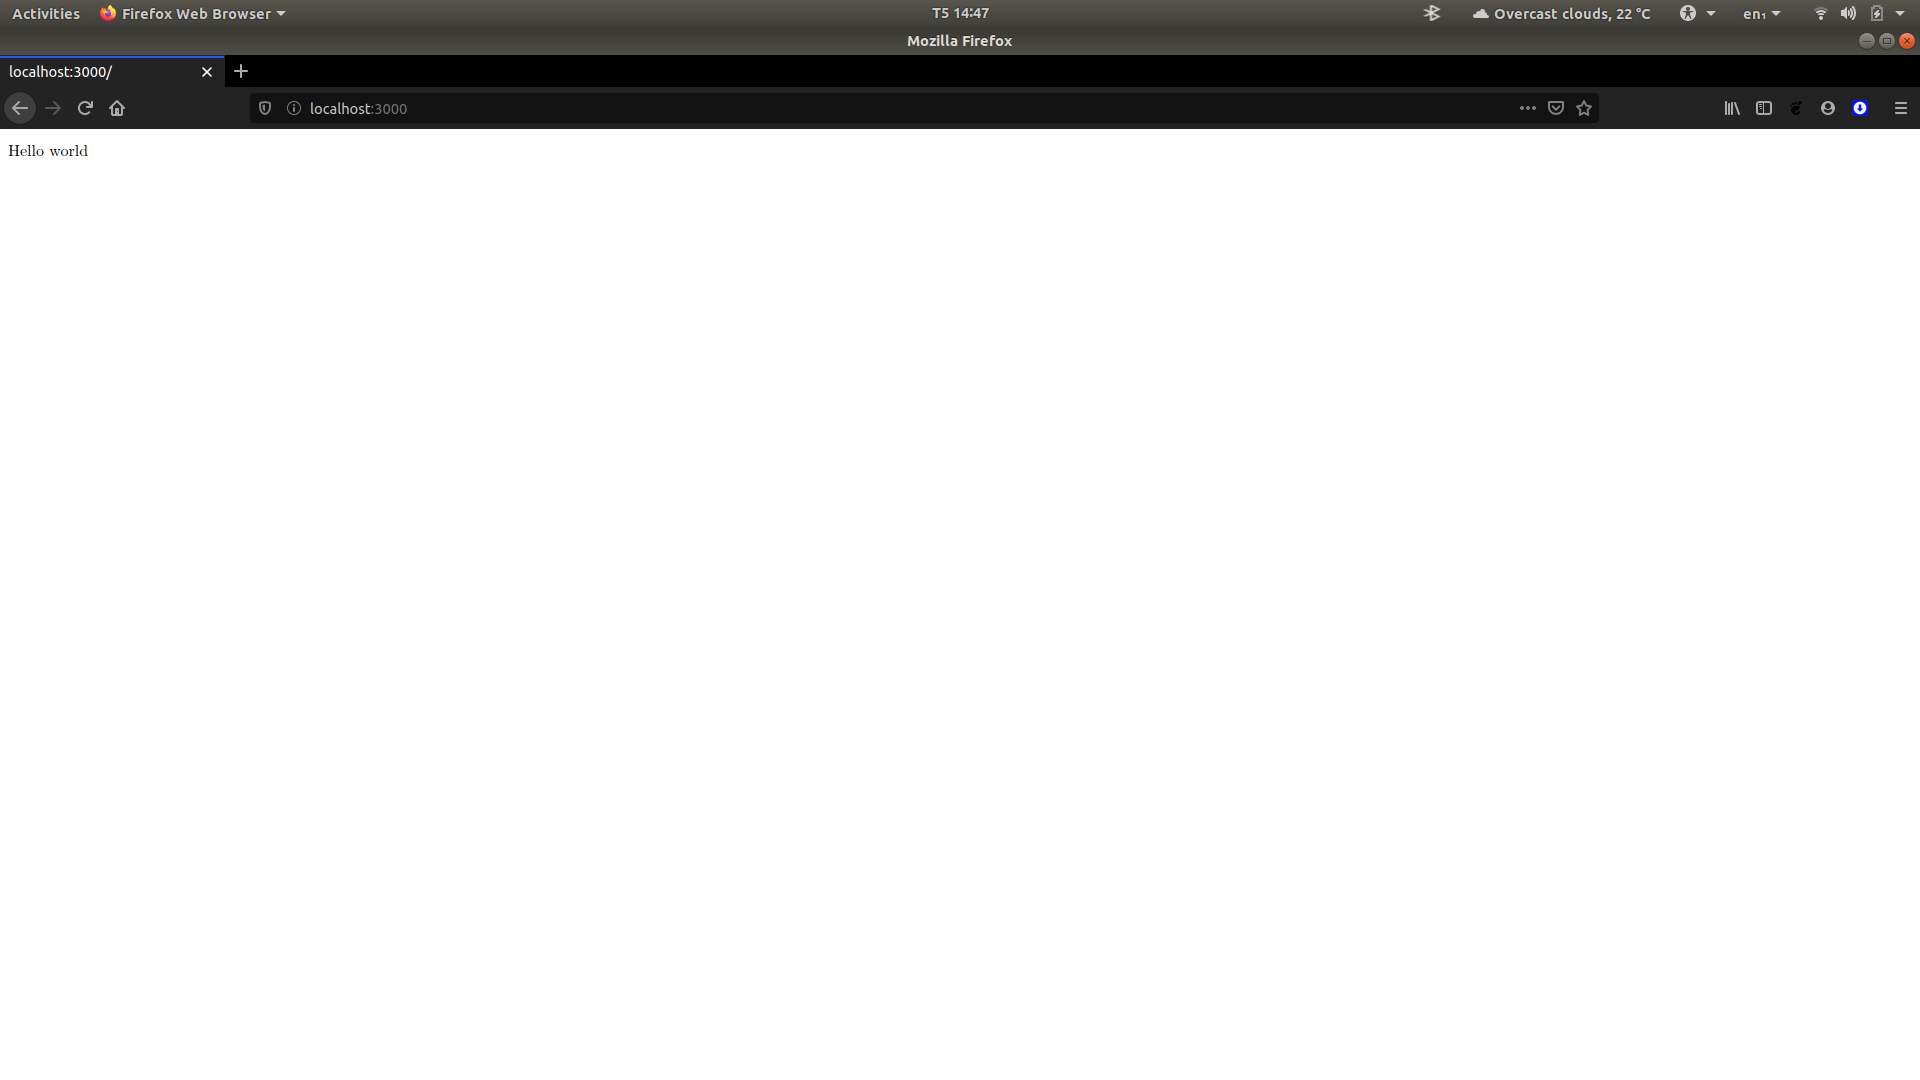
\includegraphics[width=\linewidth]{mess-on-port-3k.png}
  		\caption{Screenshot of the web browser}
  		\label{fig:hello}
	\end{figure}
	\newpage
	\section{Try Reload the Web Browser After Added socket.io}
	The console does not change since it is stil 1 'user' that conected to print hello world
	\begin{figure}[h!]
  		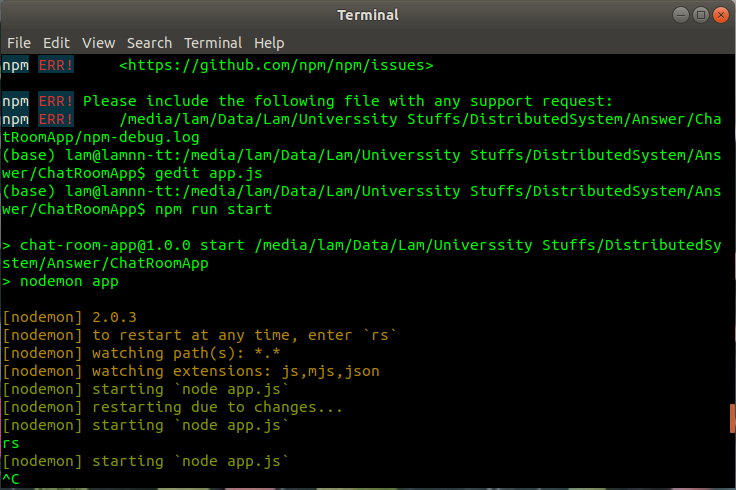
\includegraphics[width=\linewidth]{reload-web-before.png}
  		\caption{Screenshot of the console after added socket.io}
  		\label{fig:console1}
	\end{figure}
	
	\section{Try Reload the Web Browser After Fixed the Route and Added Style}
	This time, there is 'New User Connected' on the console
	\begin{figure}[h!]
  		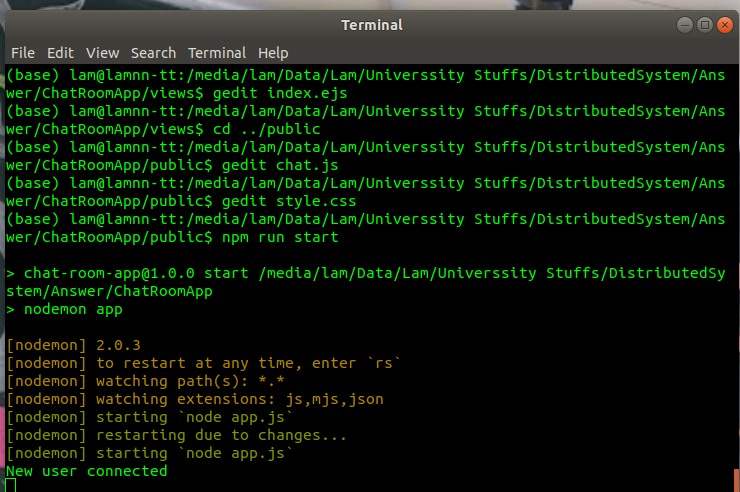
\includegraphics[width=\linewidth]{reload-web-after.png}
  		\caption{Screenshot of the console after fixed route and added style}
  		\label{fig:console2}
	\end{figure}
	
	\section{End Product}
	When 1 user is typing somthing on his or her instance, other people can see the line '$<$username$>$ is typing a message..' on top of the chatbox, in italic. When said user send the message, everyone will see a box with content as $<$username$>$: $<$message$>$ in blue.
	\begin{figure}[h!]
		\centering
  		\begin{subfigure}[b]{0.4\linewidth}
  		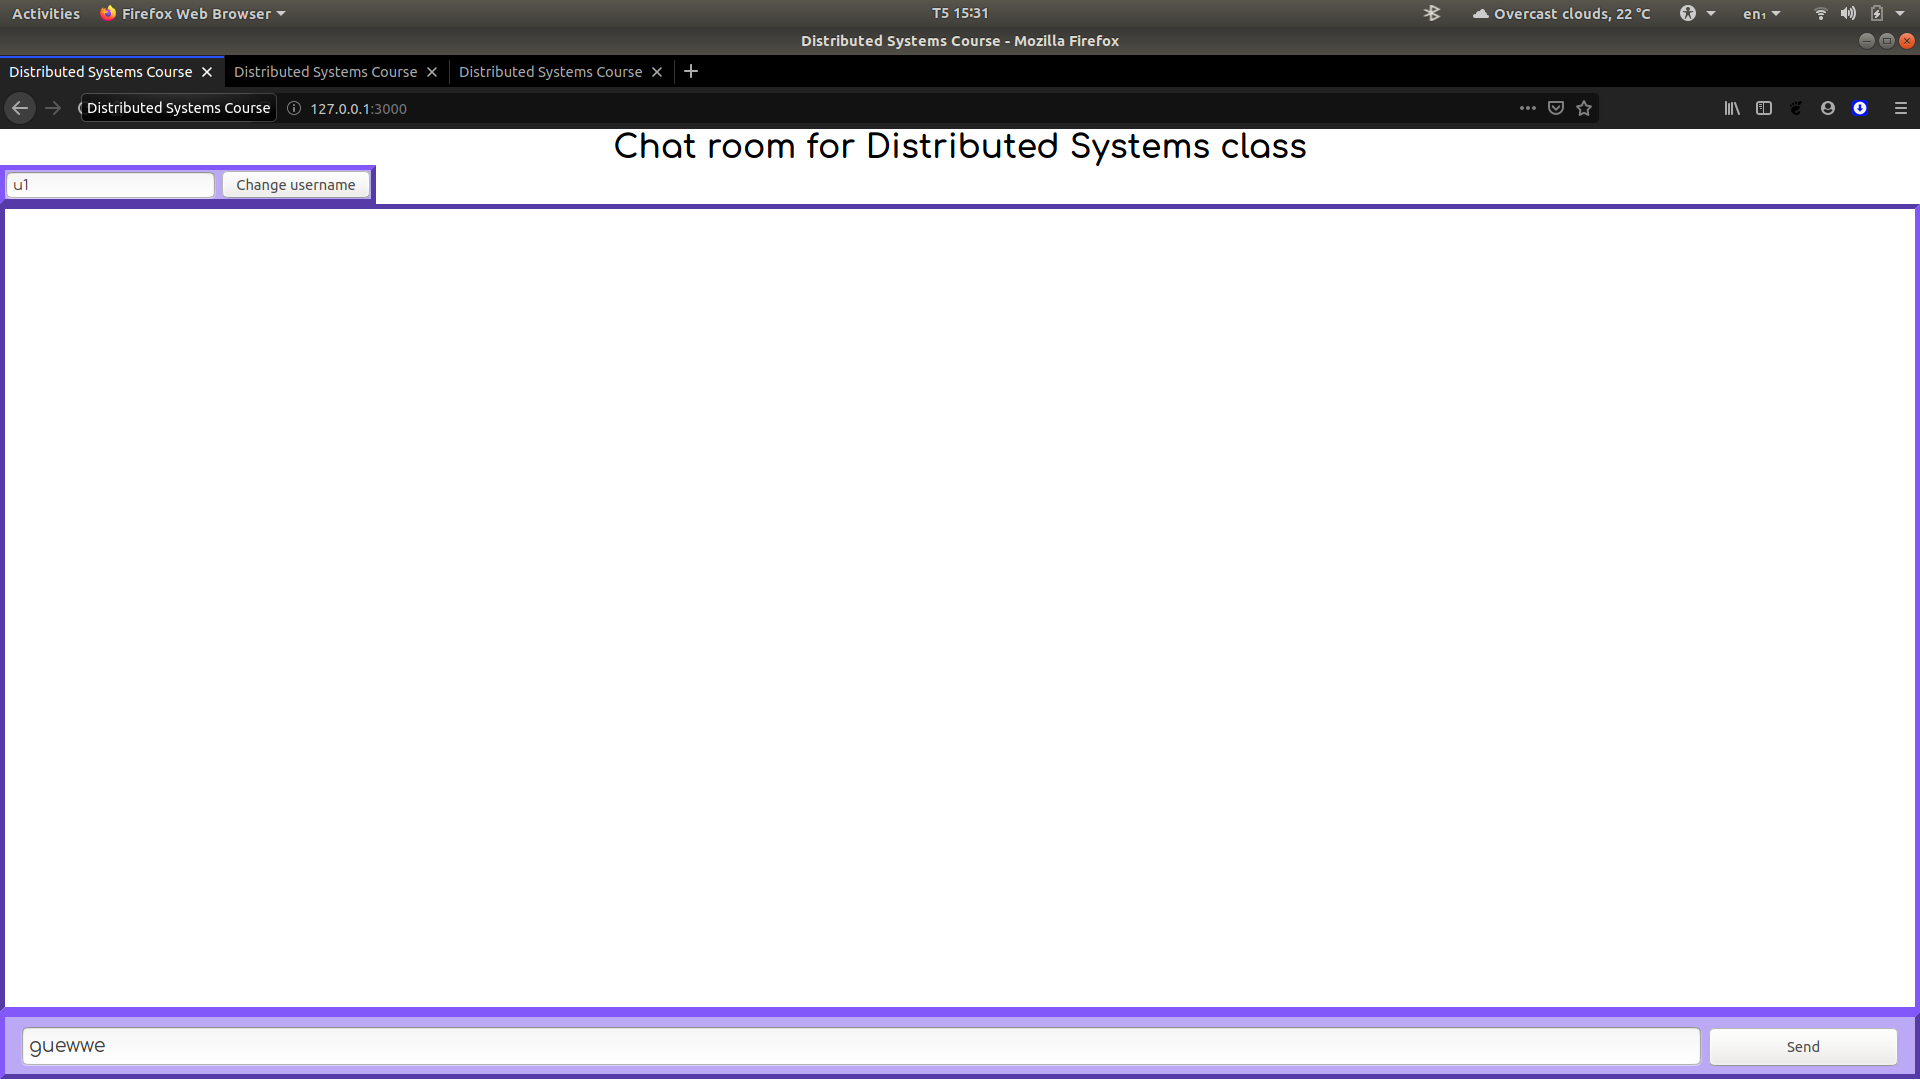
\includegraphics[width=\linewidth]{u1-type-notsend.png}
    		\caption{User u1 is typing}
  		\end{subfigure}
  		\begin{subfigure}[b]{0.4\linewidth}
    		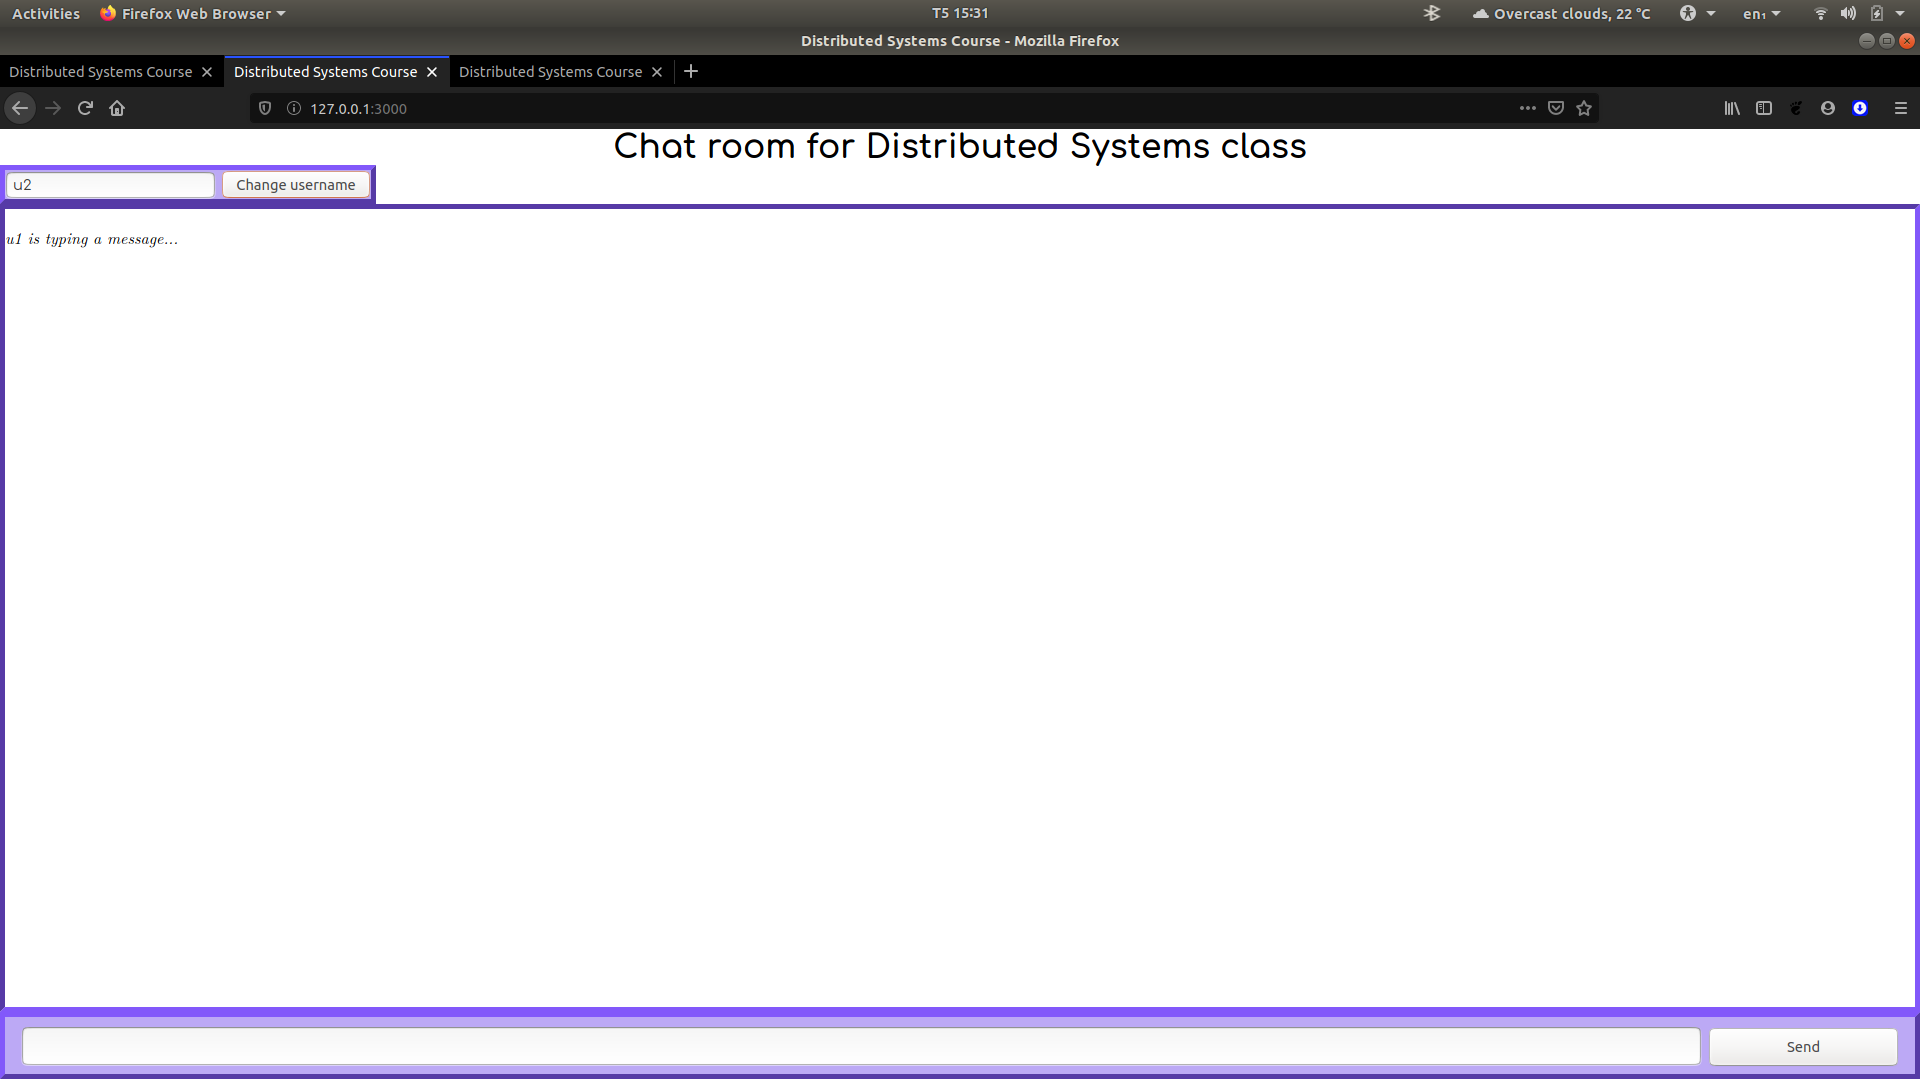
\includegraphics[width=\linewidth]{u2-notsend.png}
    		\caption{At the same time, on user u2's instance}
  		\end{subfigure}
  		\begin{subfigure}[b]{0.4\linewidth}
    		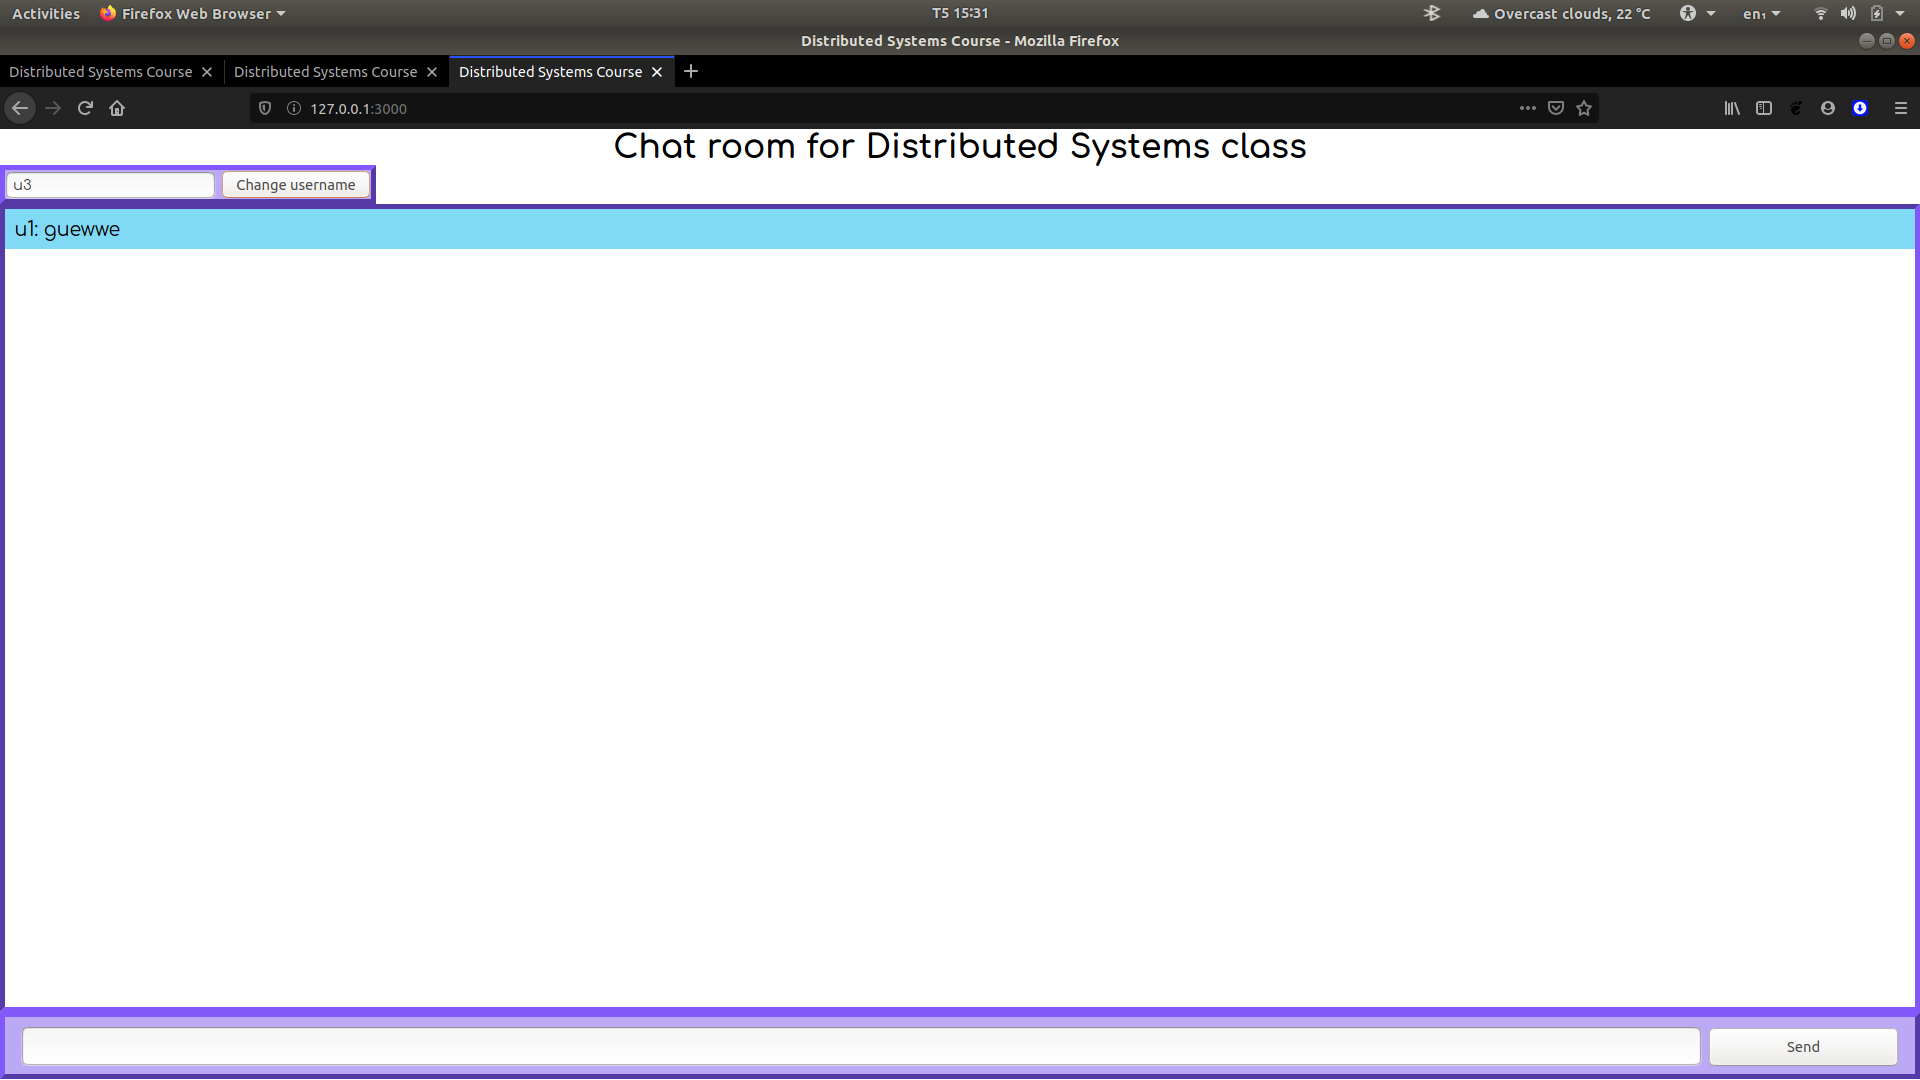
\includegraphics[width=\linewidth]{u3-aftersend.png}
    		\caption{After u1 hit send, on u3's instance}
  		\end{subfigure}
  		\caption{Final Product}
  		\label{fig:chat}
	\end{figure}
	
\end{document}